\documentclass{scrartcl}

\usepackage{hyperref}
\usepackage{graphicx}

\begin{document}

\title{Gradr: Scalable Automatic Grading for Everyone}
\subtitle{System Overview, Load Testing, and Experience Report}
\author{Kyle Dewey, Jared Roesch, and Daniel Spokoyny}
\date{December 15, 2014}

\maketitle

\section{Introduction}
Gradr is a cloud-based system for automatically building, testing, and grading student solutions to class assignments.
The ultimate end goal of Gradr is to be used in MOOC-like settings, where it acts as a student submission system, an automated feedback generator, and an automated grader.

The goals of Gradr bring up a number of technical challenges relating to scalability.
Not only do the number of submissions become large in this setting, erratic usage patterns are a problem (e.g., many submissions just before a deadline).
For this reason, Gradr must be designed in a way which is not only scalable (for the overall load), but elastic --- we should be able to dynamically add and remove system resources as needed.

\section{System Overview}
Gradr is implemented as a distributed system with multiple components, which allows for concerns to be separated out and for horizontal scaling to be inserted at key points.
Where possible, we have used components from elsewhere which satisfy our needs.
A description of the different components in Gradr follows:

\begin{description}
  \item[GitHub~\cite{github}] \hfill \\
    A publicly-available hosting service for code repositories, focused around the \texttt{git}~\cite{git} revision control system.
    GitHub stores student solutions, lifting the burden of code storage off of Gradr.
    GitHub also informs the rest of the Gradr system whenever code is submitted (via a typical \texttt{push}), triggering downstream building to occur.

  \item[Postgres~\cite{postgres}] \hfill \\
    A popular relational database engine, which serves to store persistent information.
    Postgres also facilitates communication between different components of Gradr, as it stores globally synchronized state.

  \item[Notification Listener] \hfill \\
    A custom component which listens for \texttt{push} notifications from GitHub via a webhook~\cite{github_webhook}.
    Whenever a student performs a \texttt{push}, GitHub performs a standard \texttt{POST} request to this service, providing:
    \begin{itemize}
      \item The unique GitHub username of the student performing the \texttt{push} (which is ultimately mapped back to a unique username in Gradr)
      \item The name of the repository the student \texttt{push}ed to (which is ultimately mapped back to a unique assignment identifier in Gradr)
      \item The branch on which the \texttt{push} occurred
    \end{itemize}
    The above information is put into the Postgres database, and is marked as pending for downstream processing.

  \item[Worker] \hfill \\
    A custom component which regularly polls the Postgres database, looking for student submissions which are marked as pending.
    The worker will first select a pending entry, and mark it as being processed.
    The worker will then download the submission from GitHub, compile it, run tests, and put the test results pack into the Postgres database, finally marking the entry as complete.
    Crucial to Gradr's design is the fact that there can exist any number of worker components at any time.

  \item[Frontend] \hfill \\
    A custom web application which students and instructors can use to view feedback on their submissions, which was derived from workers.
    Much like workers, there can exist multiple frontend components at any time.
\end{description}

A graphical representation of these components, along with the data flow between them, can be seen in Figure~\ref{fig:system_overview}.

\begin{figure}[h!]
  \begin{center}
    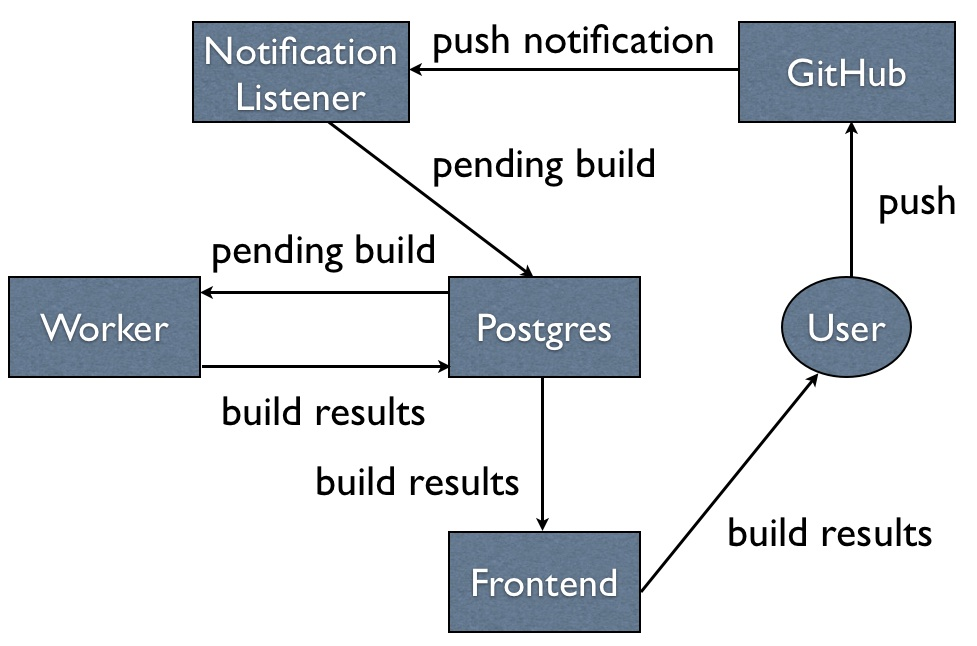
\includegraphics[scale=0.45]{non_graph_images/system_overview.jpg}
  \end{center}
  \caption{Diagram of overall Gradr architecture, along with data flow between components and the user}
  \label{fig:system_overview}
\end{figure}

\section{Load Testing}
\subsection{Critical Paths}
\label{sec:critical_paths}

With respect to how Gradr is intended to be used, we identify three critical paths:

\begin{itemize}
  \item The process of polling pending builds from the database and putting results into the database
  \item The process of putting a pending build into the database from a GitHub \texttt{push} notification
  \item Users viewing build results on the frontend
\end{itemize}

The rest of the report focuses on the first of these tasks, as it is expected to be the most executed part of the architecture.

\subsection{Experimental Setup}
For all experimenents, we used RDS~\cite{rds} with a single \texttt{db.ts.small} instance.
As we focus only on builds, the number of notification listeners and frontend systems was kept constant at one.

Submitted code was carefully controlled, and kept uniform for the duration of individual experiments.
The actual submitted code can be found at \url{https://github.com/kyledewey/test-gradr}.
Two student submissions were used, described below:
\begin{description}
  \item[\texttt{sleephalf}] \hfill \\
    Under the \texttt{sleephalf} branch, the code when run will sleep for a half of a second, and then print out some fake test results.

  \item[\texttt{sleep3}] \hfill \\
    Under the \texttt{sleep3} branch, the code when run will sleep for a three seconds, and then print out some fake test results.
\end{description}

The reason why both submissions simply sleep as opposed to doing a real code build and test cycle is because this cuts out large amount of variability between individual instances.
We can know for sure that the build should take a precise, fixed amount of time under all circumstances.
This allows us to focus in on communication overhead within the system and other related issues.
While this unit time property is unrealistic, in practice, issues pertaining to CPU or IO-intensive builds could be simply adjusted by using bigger instance types, and these are not issues fundamental to Gradr itself.

Workers were distributed in five different ways, described below:
\begin{description}
  \item[Single Small] \hfill \\
    A single worker process runs on a single \texttt{t2.small} EC2~\cite{ec2} instance.

  \item[Two Small] \hfill \\
    Each of two \texttt{t2.small} EC2 instances run a single worker process.

  \item[Four Small] \hfill \\
    Each of four \texttt{t2.small} EC2 instances run a single worker process.

  \item[One Large] \hfill \\
    Two worker processes run on a single \texttt{m3.large} EC2 instance.

  \item[Two Large] \hfill \\
    Each of two \texttt{m3.large} EC2 instances run two worker processes.
\end{description}

For all experiments, we sent 100 push notifications of whichever chosen repository and branch to the notification listener, initially with no running workers.
Once all notifications were sent, workers were started in parallel in the formation according to whichever AWS configuration was chosen.
While experiments are running, we measure the number of pending builds (queue length) over time.
Once an experiment finishes, we determine the average amount of time each build took, starting from the point where a build was selected for processing and ending with the time the results were posted.

The goal with measuring the queue length over time is to identify any anomalies in communication.
We would expect in all cases a straight line, and any other shape would indicate issues related to predictability, such as non-constant communication overhead.

The goal with measuring the average time of each build is to determine the overall overhead of the system itself.
Since the time each build takes is known in advance, we know that any additional time is purely overhead of our system.

The goal with varying the instance configuration is to identify any sort of unseen computational and network bottlenecks, along with measuring scalability of the system.
If the worker process is CPU-intensive independent of the actual student code, then this would reveal itself as bigger instance types performing better than smaller instance types.
Additionally, in a perfectly scalable environment we would expect to see that twice as many worker threads can clear a queue of pending builds in half the time, and so on.
This would not be true of a high-contension situation, and would be strong cause to optimize.

\subsection{Results and Discussion}
\label{sec:results_discussion}

We breakdown the results according to the type of the code submission used (either \texttt{sleephalf} or \texttt{sleep3}).

\subsubsection{\texttt{sleephalf}}
\label{sec:sleephalf}
Charts showing the queue length reduction over time are shown below in Figures~\ref{fig:sleephalf_one_small_queuelength}, \ref{fig:sleephalf_two_small_queuelength}, \ref{fig:sleephalf_four_small_queuelength}, \ref{fig:sleephalf_one_large_queuelength}, and~\ref{fig:sleephalf_two_large_queuelength}.

\begin{figure}[h!]
  \begin{center}
    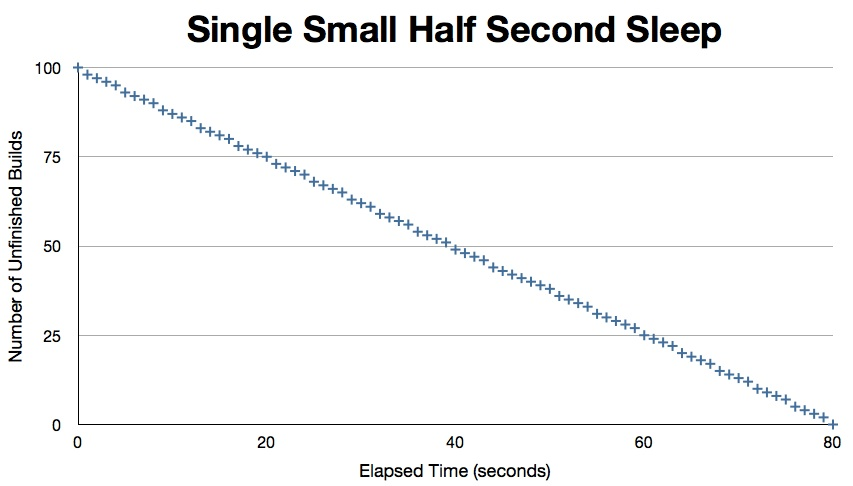
\includegraphics[scale=0.45]{raw_data/sleep0.5/one_small/graph.jpg}
  \end{center}
  \caption{Single Small Half Second Sleep}
  \label{fig:sleephalf_one_small_queuelength}
\end{figure}

\begin{figure}[h!]
  \begin{center}
    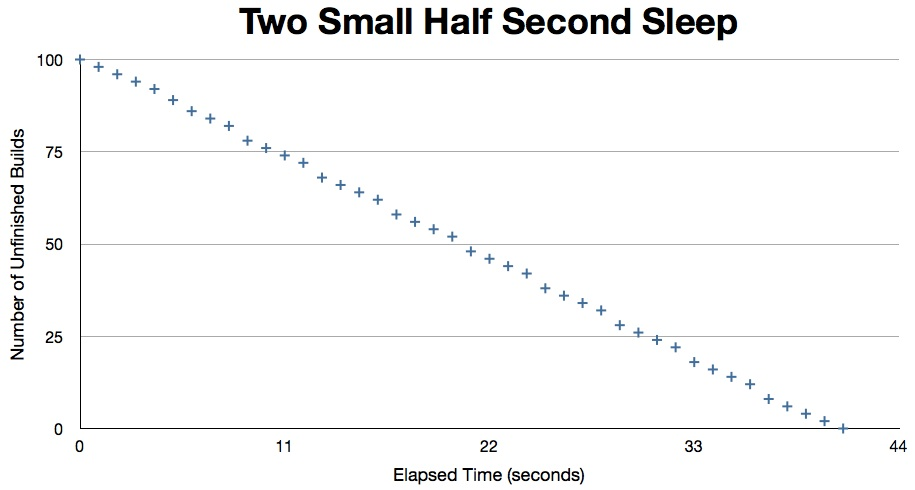
\includegraphics[scale=0.45]{raw_data/sleep0.5/two_small/graph.jpg}
  \end{center}
  \caption{Two Small Half Second Sleep}
  \label{fig:sleephalf_two_small_queuelength}
\end{figure}

\begin{figure}[h!]
  \begin{center}
    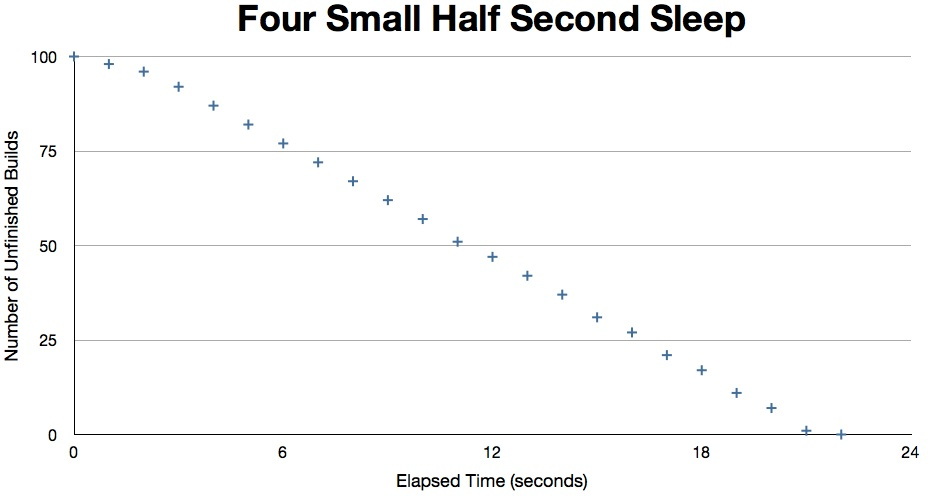
\includegraphics[scale=0.45]{raw_data/sleep0.5/four_small/graph.jpg}
  \end{center}
  \caption{Four Small Half Second Sleep}
  \label{fig:sleephalf_four_small_queuelength}
\end{figure}

\begin{figure}[h!]
  \begin{center}
    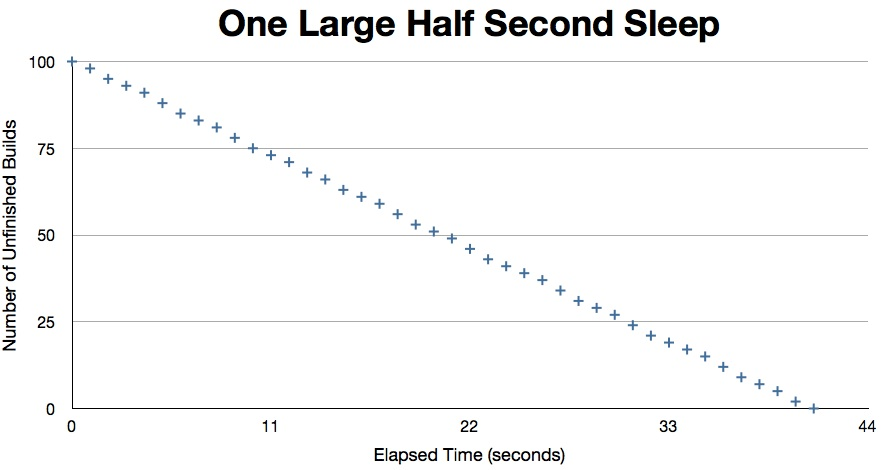
\includegraphics[scale=0.45]{raw_data/sleep0.5/one_large/graph.jpg}
  \end{center}
  \caption{One Large Half Second Sleep}
  \label{fig:sleephalf_one_large_queuelength}
\end{figure}

\begin{figure}[h!]
  \begin{center}
    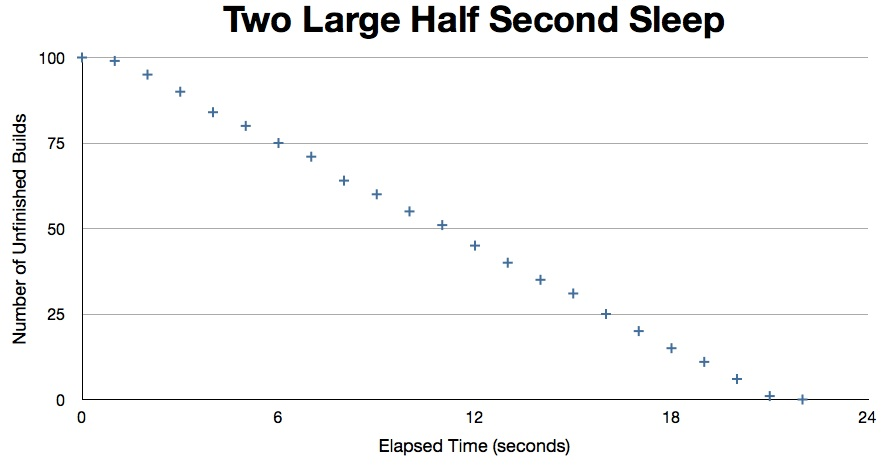
\includegraphics[scale=0.45]{raw_data/sleep0.5/two_large/graph.jpg}
  \end{center}
  \caption{Two Large Half Second Sleep}
  \label{fig:sleephalf_two_large_queuelength}
\end{figure}

As shown, in nearly all cases, the trend is a downward straight line, illustrating both that the system is predictable and communication overhead is constant.
There is a slight curve at the end of the trend in Figure~\ref{fig:sleephalf_two_large_queuelength}, which is explained by the fact that queue length results are captured with only one-second granularity and so the line likely ended sooner in reality.
The slight curve at the start of Figure~\ref{fig:sleephalf_two_large_queuelength} can be explained by the fact that workers were starting only approximately in parallel --- there were slight delays in starting occassionally.
As such, it seems likely that a subset of the workers started processing builds before all the workers started, resulting in fewer than expected builds per second.

We also measured the global amount of time taken to process all builds between the different worker configurations, shown below in Figure~\ref{fig:sleephalf_all}.

\begin{figure}[h!]
  \begin{center}
    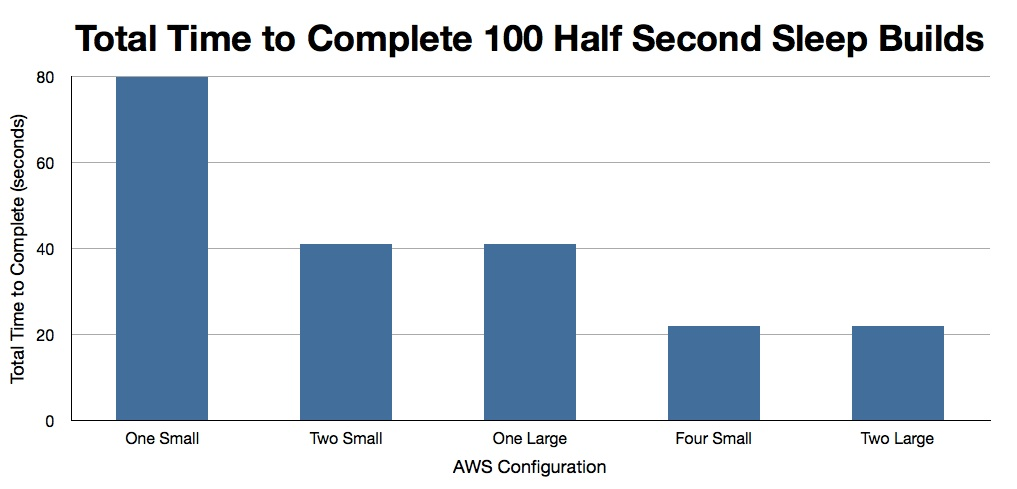
\includegraphics[scale=0.45]{raw_data/sleep0.5/time_to_complete_all.jpg}
  \end{center}
  \caption{Time to complete all builds across different worker configurations, where each build slept for half of a second}
  \label{fig:sleephalf_all}
\end{figure}

As shown, the only factor which is relevant to decreasing the amount of time taken to perform all the builds is the number of worker threads processing data.
Both the \textbf{Two Small} and \textbf{One Large} configurations take approximately the same amount of time, and similarly the \textbf{Four Small} and \textbf{Two Large} configurations, because the number of worker threads is the same --- two and four, respectively.
Additionally, the amount of time taken for \textbf{Two Small} is almost exactly half of \textbf{One Small}, and similarly the amount of time taken for \textbf{Four Small} is almost exactly half of \textbf{One Large}.
These facts indicate that we have perfect horizontal scaling of workers, at least for relatively small numbers of worker processes.

We also measured the average amount of time taken from the point when a pending build was selected from the database and the point when build results were placed in the database.
This was done for all aforementioned worker configurations.
The results are shown below in Figure~\ref{fig:sleephalf_each}.

\begin{figure}[h!]
  \begin{center}
    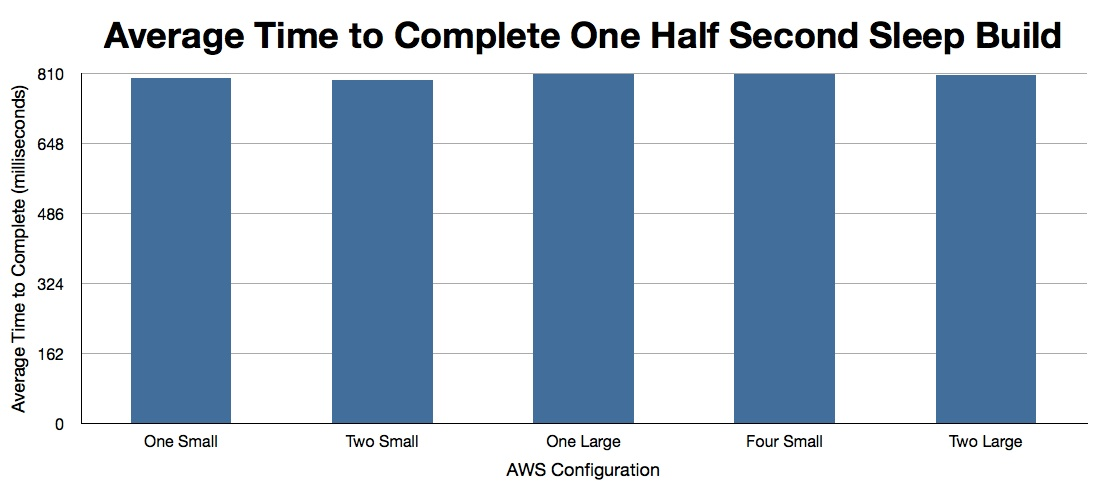
\includegraphics[scale=0.45]{raw_data/sleep0.5/time_to_complete_each.jpg}
  \end{center}
  \caption{Average time to complete a single build across different worker configurations, where each build slept for half of a second}
  \label{fig:sleephalf_each}
\end{figure}

As shown, the effect of the configuration had essentially no impact on the amount of time taken for a build, which was expected given the fact that the builds simply sleep.
Additionally, we can use this data to measure the overhead of Gradr itself.
We can see that builds take approximately 800 milliseconds.
Combining this with the fact that builds simply sleep for 500 milliseconds, we can estimate Gradr's overhead to be approximately 300 milliseconds per build.
The vast majority of this time is spent downloading code from GitHub, and was around 200 milliseconds in informal experimentation.
This shows that Gradr workers have overall very low overhead, and there is not much that can be done to improve this.

\subsubsection{\texttt{sleep3}}
\label{sec:sleep3}

Charts showing the queue length reduction over time for the \texttt{sleep3} build are shown below in Figures~\ref{fig:sleep3_one_small_queuelength}, \ref{fig:sleep3_two_small_queuelength}, \ref{fig:sleep3_four_small_queuelength}, \ref{fig:sleep3_one_large_queuelength}, and~\ref{fig:sleep3_two_large_queuelength}.

\begin{figure}[h!]
  \begin{center}
    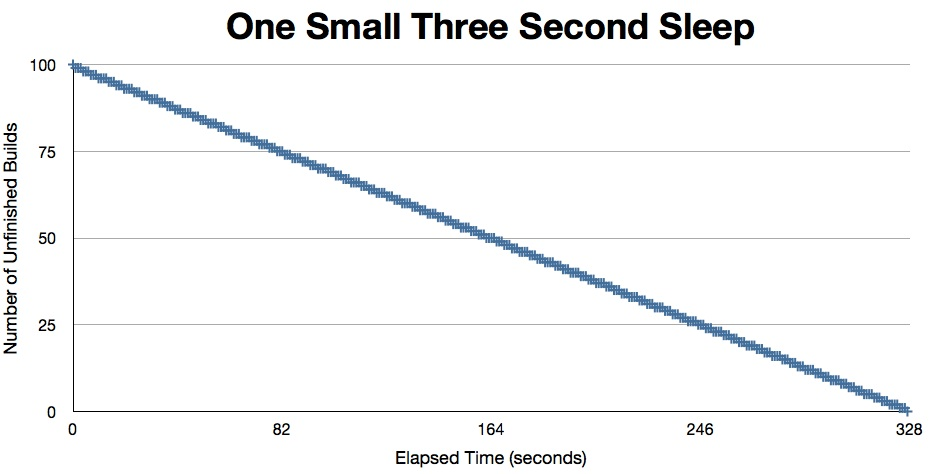
\includegraphics[scale=0.45]{raw_data/sleep3/one_small/graph.jpg}
  \end{center}
  \caption{Single Small Three Second Sleep}
  \label{fig:sleep3_one_small_queuelength}
\end{figure}

\begin{figure}[h!]
  \begin{center}
    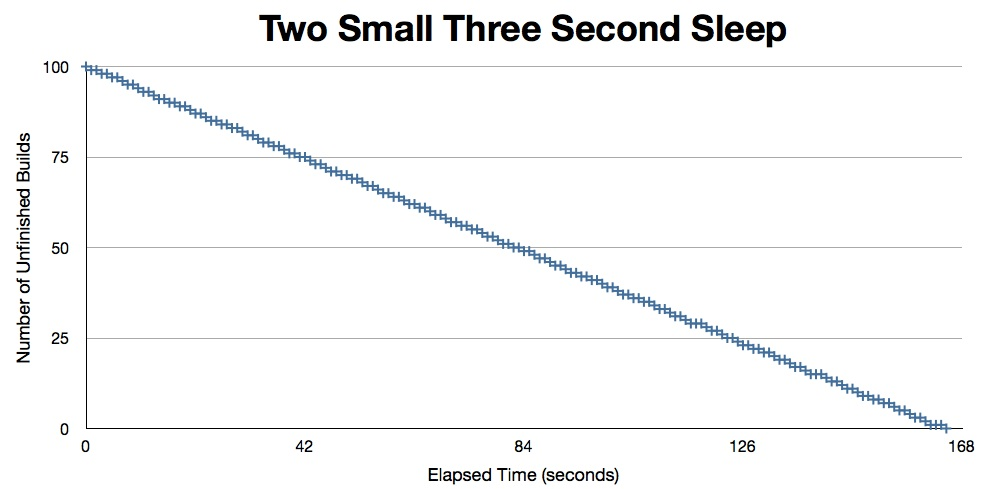
\includegraphics[scale=0.45]{raw_data/sleep3/two_small/graph.jpg}
  \end{center}
  \caption{Two Small Three Second Sleep}
  \label{fig:sleep3_two_small_queuelength}
\end{figure}

\begin{figure}[h!]
  \begin{center}
    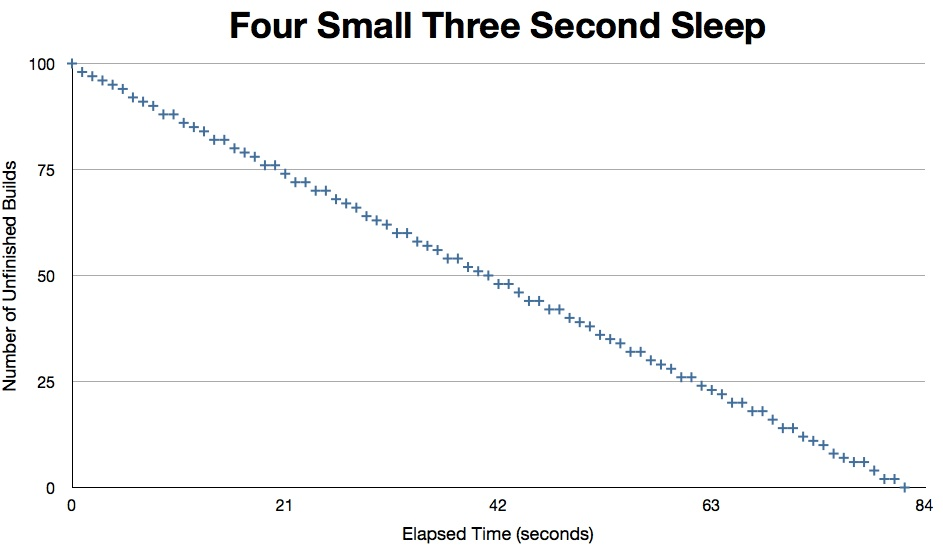
\includegraphics[scale=0.45]{raw_data/sleep3/four_small/graph.jpg}
  \end{center}
  \caption{Four Small Three Second Sleep}
  \label{fig:sleep3_four_small_queuelength}
\end{figure}

\begin{figure}[h!]
  \begin{center}
    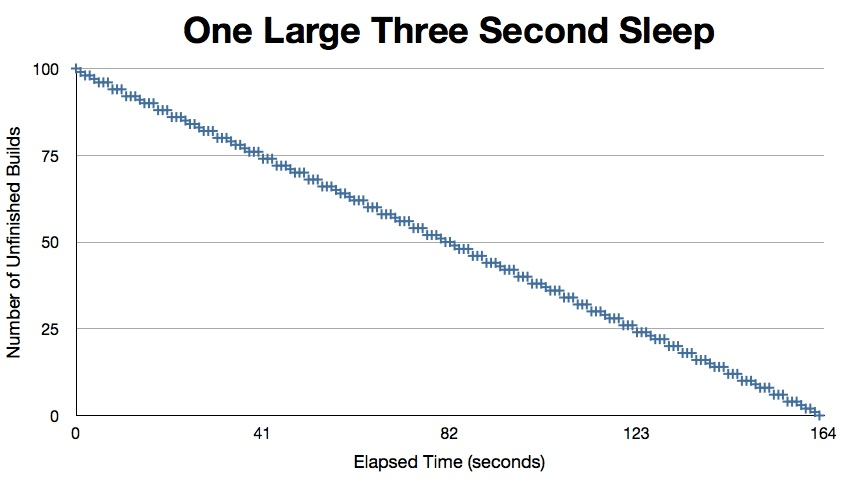
\includegraphics[scale=0.45]{raw_data/sleep3/one_large/graph.jpg}
  \end{center}
  \caption{One Large Three Second Sleep}
  \label{fig:sleep3_one_large_queuelength}
\end{figure}

\begin{figure}[h!]
  \begin{center}
    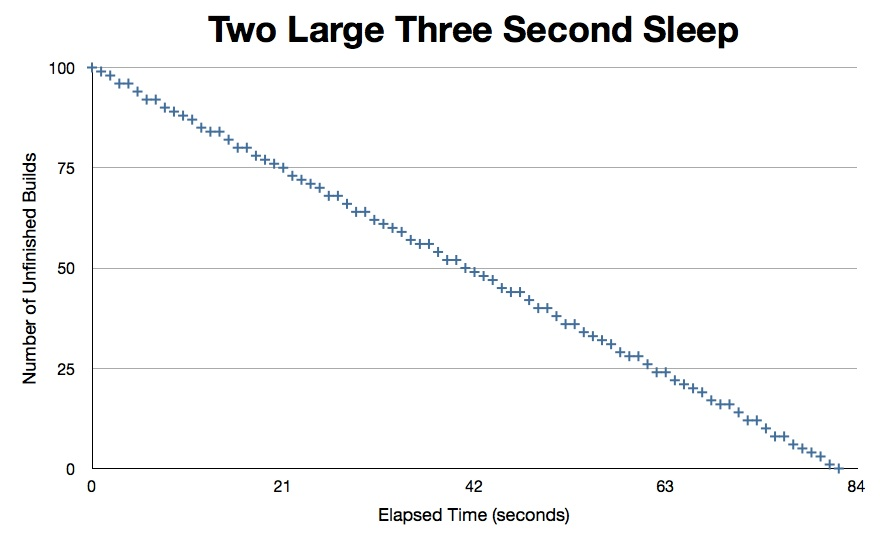
\includegraphics[scale=0.45]{raw_data/sleep3/two_large/graph.jpg}
  \end{center}
  \caption{Two Large Three Second Sleep}
  \label{fig:sleep3_two_large_queuelength}
\end{figure}

The above results are extremely similar to those of Section~\ref{sec:sleephalf}, and so we draw the same conclusions as before.

We also measured the global amount of time taken to process all builds between the different worker configurations, shown below in Figure~\ref{fig:sleep3_all}.

\begin{figure}[h!]
  \begin{center}
    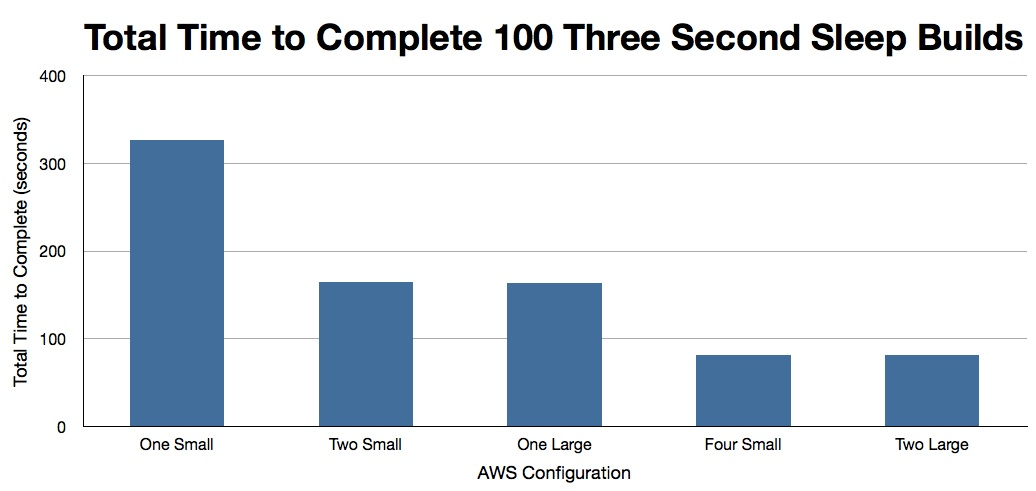
\includegraphics[scale=0.45]{raw_data/sleep3/time_to_complete_all.jpg}
  \end{center}
  \caption{Time to complete all builds across different worker configurations, where each build slept for three seconds}
  \label{fig:sleep3_all}
\end{figure}

Once again, we draw the same conclusions from Figure~\ref{fig:sleep3_all} as done in Section~\ref{sec:sleephalf}, as the shape is nearly identical.

As for the average time taken for each build, this data is shown below in Figure~\ref{fig:sleep3_each}.

\begin{figure}[h!]
  \begin{center}
    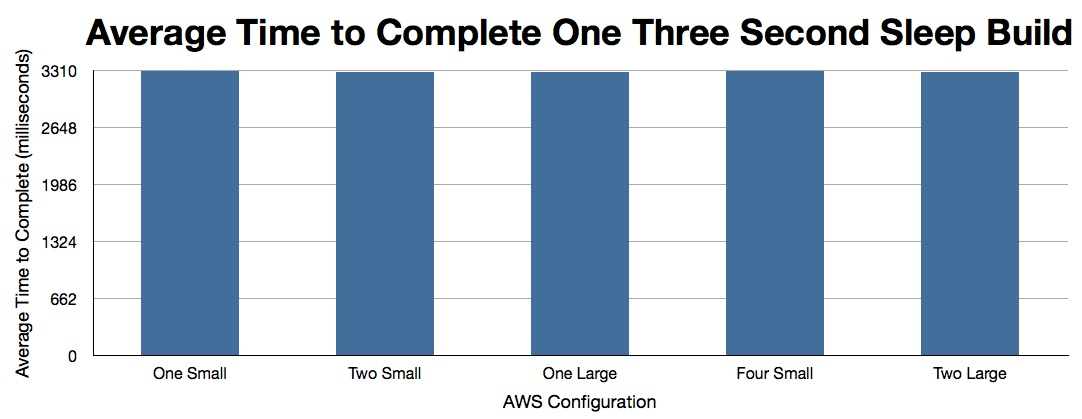
\includegraphics[scale=0.45]{raw_data/sleep3/time_to_complete_each.jpg}
  \end{center}
  \caption{Average time to complete a single build across different worker configurations, where each build slept for three seconds}
  \label{fig:sleep3_each}
\end{figure}

Once again, the total time taken did not significantly vary between the different worker configurations, leading us to conclude that there is no hidden system overhead.
The prior estimation of 300 milliseconds of system overhead also remains consistent, given that builds sleep for 3000 milliseconds (three seconds) and generally take 3300 milliseconds to complete.

Overall, we conclude that the critical path involving workers, which is likely to be the most stressed path, is both highly performant and scalable.

\subsection{Load Testing Other Critical Paths}
\label{sec:load_testing_other_critical_paths}

Some attempt was also made at stressing the path from GitHub to the notification listener.
For this experiment, 10 threads sequentially kept sending push notifications directly to the notification listener, bypassing GitHub on the assumption that GitHub may throttle back notifications.
A visible connection backlog was set to one, in an attempt to force a \texttt{POST} failure.
Even under these conditions, we were unable to get a failure to occur.
This seems to be due to two major reasons.
For one, each \texttt{POST} can be processed quite rapidly, within about 30 milliseconds including interactions with Postgres.
This time is independent of the size of the database, thanks to indecies of appropriate columns in the database.
Indeed, looking at the server, even on a \texttt{t2.small} instance the notification listener process only uses approximately 6\% of the CPU, indicating that 10 parallel senders is not enough to put sufficient strain on it.
An additional reason is that with the \texttt{HTTP} server we are using (\texttt{hyper}~\cite{hyper}), a curory glance at some of the source code hints that there may be attempts to perform parallel connections, even though this is not supposed to be case according to its documentation.
If this is true, it would take an enourmous amount of stress to start seeing failures.

As for the frontend, there has not been sufficient effort on load testing it due primarily to lack of time.
However, in Section~\ref{sec:performance_improvements}, we do discuss possible issues and solutions in this critical path.

\section{Possible Further Improvements}
\label{sec:performance_improvements}

This section describes possible improvements which can be made to individual components.
While the primary focus is on improving scalability with respect to the critical paths discussed in Section~\ref{sec:critical_paths}, there are some other miscellaneous improvements of interest as well.

\subsection{Frontend}
\label{sec:improve_frontend}

Currently, while multiple instances of the frontend can be run in parallel, they are not unified behind a single URL due to the lack of a proper load balancer.
An obvious improvement here is use a load balancer, which should address frontend issues.
While this alone is likely insufficient for a typical app, with Gradr, we suspect that this would get us a long way.
The primary purpose of the frontend is to communicate build results to the user, and the only intended modifications are infrequent, relatively inexpensive administrative-style tasks like adding classes and assignments.
As such, the frontend is only read-centric, and in a very particular way, so contention here with the database is expected to be low.

Even if database contension here starts increasing, there is a lot that could be done to amend this situation.
We observe that once results are uploaded to the database, the entry does not change, nor do the results.
As such, Postgres read replicas should do well here.
Moreover, we could be much more intelligent, and store the results in an auxilliary place like S3~\cite{s3} or DynamoDB~\cite{dynamodb}.
With such a setup, the database exists purely to store metadata (which is small and needs strong guarantees about synchronization), and the auxilliary store exists purely to store results (which are large, unchanging, and are quite amenable to an eventually-consistent model).

\subsection{Notification Listener}
While Section~\ref{sec:load_testing_other_critical_paths} demonstrated that the notification listener does not currently have any problems responding to moderate numbers of requests, this is not to say that improvements should not be made.
In fact, there is quite a bit of room for improvement here.
One obvious improvement is to serve requests in parallel, which would be fairly easy to do thanks to the way the code is architected.
Beyond this simple change, as described with the frontend in Section~\ref{sec:improve_frontend}, we could put a load balancer in front of the notification listener.

One other potential improvemnent for the notification listener involves how it interacts with the database.
Currently, the notification listener must update three separate tables upon the insertion of a single build, which is performed in a transaction which spans several queries.
This portion of the system is ripe for denormalization~\cite{denormalization}, which would allow us to perform the update in a single query.
Not only would this mean a less complex transaction, it most likely would improve performance.

\subsection{Worker}
\label{sec:improve_worker}

As shown in Section~\ref{sec:results_discussion}, there is not a whole lot that can be improved scalability-wise when it comes to workers.
However, there is still more that could be done here.
For one, while workers can be currently added dynamically without a problem, removing workers is more difficult.
This is because workers ``take'' a pending build from the database by marking a special field as being in-progress, and workers know not to take in-progress builds.
This means that if a worker marks a field as in-progress and subsequently crashes before uploading the results, the build will never be completed.
Not only does this make removing workers a pain, it means that they are not very fault-tolerant.

To address this issue, SQS~\cite{sqs} would be a much better choice than Postgres for selecting builds.
With SQS, in order to remove an item from a queue permanently, one must both dequeue and mark it as complete to SQS.
If a thread dequeues but fails to mark it complete, then the item will reappear in the queue after a configurable amount of time.
This means that in the crash scenario, we would dequeue but never mark it as complete, so the build would reappear to other workers for processing.
As long as workers only mark a build as complete when the results have been uploaded, this fault tolerance issue will disappear.
(Workers can also ask SQS for more time, and indicate that they have not crashed in doing so.)

Another problem with workers relates to both configurability and security.
Currently, it is assumed that all assignments in the system can be compiled and run with the same makefile, which is unrealistic.
More importantly, builds are performed without any sort of sandboxing, so it would be relatively easy for a malicious student to take control of a worker.
This would be disasterous, as with some ingenuity the student could gain access to the database, and in so doing take control over nearly the entire system and its data.

It turns out that both these problems can be addressed using the same tool: Docker~\cite{docker}.
Docker allows for virtualization on top of Linux, and can prevent access to the Internet or to the rest of the filesystem.
This would make it so that even if a malicious student were to take control, they would only take control of a highly restricted slice.
Docker would also allow instructors to assemble their own custom environments on a per-assignment basis, allowing for not just custom makefiles, but even things like arbitrary input files and compilers with specific versions.
While the use of Docker would likely increase the amount of time it would take to process individual builds, the benefits are clear.

\subsection{On the Need for a Relational Database}
As discussed in~\ref{sec:improve_frontend}, test results are amenable to eventually-consistent database models.
It turns out that this is true for most data in Gradr --- classes, assignments, and users, the primary kinds of non-test data, all have the property of being rarely updated.
As such, moving this to an eventually-consistent datastore should not be a huge burden.
In fact, currently the only part of the system which truly relies on the consistency guarantees is that of the worker thread, which needs to be able to lock a pending build while it is being processed.
As described in Section~\ref{sec:improve_worker}, this is better-suited for SQS~\cite{sqs} anyway.
With this in mind, Gradr has very high potential to scale to very large proportions.

\section{Conclusions}

Gradr is a distributed automated feedback and grading system, one with a highly scalable architecture.
Core components have withstood load testing, and has demonstrated perfect horizontal scalability.
Testing has also shown that the system imparts only a minute amount of overhead, typically only around 300 milliseconds.
While these results are quite impressive, there are still a multitude of improvements which could be made not only for scalability, but for general usability and security.

\appendix

\section{Experience Report}

This section details various lessons learned regarding how Gradr was implemented.
These are not directly relevant to Gradr itself or to Gradr's scalability and performance, but they are considered nonetheless interesting and so have been included.

\subsection{On the Usage of the Rust Programming Language}
While the frontend is implemented in Ruby~\cite{ruby} and Rails~\cite{rails}, the notification listener and the worker are implemented in the Rust programming language~\cite{rust}.
Rust is much more like C than Ruby, being a statically-typed systems programming language which ultimately compiles down to machine code.
However, unlike C code, Rust code has strong, statically-known properties pertaining to memory safety, including (but not limited to):
\begin{itemize}
  \item No \texttt{null} pointer dereferences (there is no \texttt{null})
  \item No dangling pointers
  \item No memory leaks (or, alternatively, no more memory leaks than those possible in Java)
  \item No data races (as in multithreaded code)
\end{itemize}
That is, by construction, well-typed Rust programs are statically known to not have any of the above problems.
This makes it a much more attractive language than C for doing systems programming.

By using Rust, we gain much stronger guarantees about the correctness of our code than possible with Ruby.
Additionally, Rust programs are not garbage collected, so theoretically they have very predictable performance.
These properties make Rust highly attractive to work with when it comes to workers, as this is arguably the most heavily executed portion of the system and is certainly the most complex.

\subsubsection{Advantages in Practice}
In practice, Rust gave us a lot of advantages which are simply not possible with most languages.
The most apparent advantage can be seen with the highly regular graphs measuring queue size in Sections~\ref{sec:sleephalf} and~\ref{sec:sleep3} --- there is no garbage collection to introduce sudden, unexpected pauses.
However, the greatest advantages were seen purely in development.
Very little of the development time was in debugging --- most everything was pure design and coding.
This was because of not only the language's static type system, but because it encourages very functional idioms.
While it supports mutable state, it is restricted so that all mutation is thread-safe by construction.
This forces the programmer to think very hard about state which is not immutable, resulting in very modular code.
The language is also very restrictive when it comes to aliasing objects, e.g., one cannot alias an object twice and then mutate it, for this could potentially lead to a data race.
Again, this forces modular design.

What is truly amazing about these restrictions is that after an initial barrier to entry is crossed (approximately one week for the writer), they become second nature.
After this point, all the fights the writer had with the compiler turned out to be subtle issues which could actually have been problematic.
The language truly makes you appreciate what you cannot due.

\subsubsection{Database Operations}
Another feature of Rust is that it supports compiler plugins which are themselves written in Rust.
This can be used to generate code at compile time for specific purposes.
In doing so, we gain many of the metaprogramming advantages common to Ruby, but with much stronger guarantees about correctness.
This feature of Rust was used extensively for a novel purpose: generation of database queries.

While Postgres bindings for Rust are available, these are still problematic because:
\begin{enumerate}
  \item There is nothing stopping the user from issuing an ill-typed query.
    For example, if a given field \texttt{f} is an integer in the database, it is still possible to pass a string.

  \item These force queries to be embedded into the code, which is poor practice if the schema may change in the future.
    Schema changes will break queries, but this can be discovered only dynamically.
\end{enumerate}

To address this problem, we developed a compiler plugin which, at compile time, will:
\begin{enumerate}
  \item Connect to a specified database
  \item Read the schema
  \item Generate schema-specific data structures, accessors, and other routines
\end{enumerate}
Using this technique, it is no longer possible to issue an ill-typed query --- this will be revealed as a Rust type error.
Additionally, if the schema changes in a way that is incompatible with what is already present (e.g., a field is renamed), then this will be revealed as another kind of Rust type error.
While the development of this plugin took a substantial amount of time, it quickly paid for itself a handful of times when the schema did change and suddenly code no longer compiled.

\subsubsection{Challenges with Rust}
There was, however, a major downside to using Rust: language instability.
Rust is under active development by Mozilla~\cite{mozilla}, and is currently in Alpha status.
As a result, an all-to-frequent phenomenon is that code which worked yesterday will not work today, as breaking changes occur frequently.
This occurred no less than four times during development, and ate up over 20 hours of developer time.
While no change forced fundamental restructuring or anything otherwise severe in Gradr, Gradr pulls in dozens of dependencies, some of which did need more significant change.
The author became a contributor to 13 unrelated projects in the process, as upstream breaks were patched.

Many of these issues should be addressed with the upcoming Beta release of Rust, which is scheduled to occur within the next month of this writing.
Additionally, while development occurred, a central repository of Rust projects was formed, which is amenable to specifying specific versions of things (as opposed to being forced to always use the most recent version).
Even so, this was a very frustrating and demotivating part of the experience.

\subsection{On the Usage of Agile Methodology}
While we had originally set out to use Agile methodology for development, this was initially hampered by time constraints which prevented much progress from occurring early on.
For the development of non-frontend components, after the first few weeks, I (Kyle) attempted to stick to a plan of incremental progress, central to Agile.
I have some mixed feelings about the experience.
I found it was excellent for getting early functionality up, and got us a prototype faster than I could have imagined.
However, after this point things became difficult.
I had put a lot of emphasis on testability, and this ended up leading to interfaces which were poisoned with testing concerns.
There was also a situation in which a focus on getting functionality up led to the accumulation of technical debt which I would not otherwise have taken on, and this amounted to wasted time.

In retrospect, on the testing end of things, I believe the major problem was not with Agile, but with the fact that I was combining a new development technique along with learning a new language.
Rust's primary method of forming abstractions, that of typeclasses, is very different from the standard OOP classes most people are familiar with.
Additionally, the sort of memory guarantees Rust provides are only possible because the type system itself forces you to think about memory a bit, and without some care this can lead to a poor separation of concerns (e.g., does it make sense to allow something to mutate a given object in general?).
The end result was some very abstract, overcomplex code, which were poisoned with bizarre memory concerns.
It would have been better to get the most simple components correct first, and then worry about how to test them.

As for the accumulation of technique debt, a better option would have been to change the objective.
The only reason the debt was accumulated is because I looked at what was in reality a soft deadline as a hard deadline, and this was unnecessary.

\section{Links}
All components of Gradr are open-sourced.
Additionally, in some places components were sectioned off into separate repositories.
These different projects are described below:

\begin{itemize}
  \item Code for communicating with the Postgres database is hosted at \url{https://github.com/jroesch/pg-typeprovider}

  \item Code for listening for notifications from GitHub (though not the entire notification listener component) is hosted at \url{https://github.com/jroesch/rust-github}

  \item The notification listener is hosted at \url{https://github.com/scalableinternetservices/GradrBackend}, under the directory \texttt{gradr\_notifications}

  \item The worker is hosted at \url{https://github.com/scalableinternetservices/GradrBackend}, under the directory \texttt{gradr\_worker}

  \item The frontend component is hosted at \url{https://github.com/scalableinternetservices/Gradr}
\end{itemize}

\bibliography{bibtex}{}
\bibliographystyle{plain}

\end{document}
